%===============================================================================%
\chapter{Processing the Data into Footfall} \label{chapter:processing}
%===============================================================================%

Chapter \ref{chapter:collection} detailed the procedure through which three distinct Wi-Fi probes based datasets were collected ranging from small controlled experiments to comprehensive national level project.
It also detailed the various uncertainties, biases and challenges that are present in these datasets and possible approaches to solve them.
Having established these, this chapter aims to devise the toolkits and methods to deal with the datasets and combine them into a data processing pipeline which can to go through the data and convert them to estimation of ambient population or footfall at the locations they were collected.

As the amount of data collected with Smart street sensor project is large from a conventional computing point of view, Section \ref{section:toolkit} starts with a review of `big data' and tries to set up a framework of evaluating the datasets from a `big data' perspective.
A brief review was conducted on the topic of 'big data and big data tools' which established a framework for investigating datasets and measuring the extent of 
`bigness' in them.
Using this framework, the datasets were evaluated in each of their dimensions to understand their nature and the challenges posed in these dimensions.
We find that the Wi-Fi based datasets are 'medium data' (as opposed to 'big data') which can benefit from customised toolkits which increases the efficiency.
After evaluating the datasets, a detailed review of tools and methods to deal with big data was conducted and the ones which are relevant and feasible for further research were picked out.
Finally a complete bespoke `toolkit' was created by pulling together and connecting all the individual tools so the data can be processed in the most efficient way.

Having designed a toolkit, Section \ref{section:processing} explores the methods that can be used by this toolkit to clean and process the data.
The major uncertainties in these datasets which were identified in the last chapter were looked in to further with the specific focus on how much they affect the datasets.
We identify - the uncertain field of measurement and MAC randomisation as the biggest sources of data.
We discussed the ways in which these problems could be solved and design methods to solved them.
We propose signal strength and its analysis as solution for enforcing the field of measurement and sequence numbers and their analysis as solution for figuring out unique devices even when they were randomised. 
We formalise these ideas into algorithms and use these on the datasets one by one to find which ones are feasible and eliminating the ones that cannot help.
Both the methods are tested extensively on the data collected from the initial survey and the pilot studies and the corresponding effectiveness in reducing errors were measured.
Finally, an alternative method to adjust long term errors quickly and efficiently in large projects such as Smart street sensors was devised and tested to provide us with footfall estimations of sufficient quality.

Finally in section \ref{section:pipeline} we combine these tools and method together to make a data pipeline which takes in the large amount of the continuous inflow of data from the smart street sensor.
This pipeline downloads, cleans, processes and stores the data.
It also post-processes the data into footfall for further analysis.
The performance and the efficiency of the pipeline is briefly discussed and compared with traditional methods.
Thus completing our journey from raw Wi-Fi probe requests data to an informed estimate of footfall at retail location all around UK.

\cleardoublepage
%==============================================================================%
% Introduction to the chapter
%==============================================================================%

\section{Data Toolkit} \label{section:toolkit}

\textsc{Big data and its analytics} promises huge benefits in terms of value realisation, cost reduction, insights but it also introduces a numerous pitfalls \cite{gandomi2015}.
With developments in information technology, mobile communications and internet of things, large assemblages of data are readily available leading to immense possibilities in research.
But when we analyse these data at such scale, we also encounter a large amount of added complexity and cost.
Hence it is important to be careful in choosing the methods and tools in dealing with big data where we should look to devise right methods and tools for the right problems.
Moreover in several disciplines, such as statistics and geography etc., the existing methods and tools are already developed for dealing with large scale data.
These methods along with improvements in hardware has made the processing big data in these disciplines possible without a major changes in workflow.
In the current environment of constant change and growth of sources of data, we cannot afford to lose the opportunity to extract information from them while trying to create a perfect, future proof approach in dealing with them.
We need to move fast with a pragmatic approach where we look at other disciplines and adopt best practices and solutions in them and develop consistent approach for our needs rather than reinventing the wheel.

%------------------------------------------------------------------------------%

In the previous chapters we looked at various methods we devised to collect and process data from Wi-Fi probe requests emitted by phones.
Though we discussed the methods conceptually, we left out the rationale behind choosing the toolkit employed to implement those methods.
In this section we elaborate the thought process and rationale behind these decisions.
We start by discussing the concept of `Big Data' in general and look at previous literature to understand its definition, nature and the challenges they pose.
Then we look at the data-sets we collected through the pilot studies and the `Smart Street Sensor' project and evaluate them in terms of the dimensions of the big data.
We also discuss the challenges faced in dealing with our dataset in detail and try to understand the requirements for devising a toolkit for it.
Finally we put together a toolkit to suit our datasets built from simple small UNIX tools. \sidenote[]{"Write programs that do one thing and do it well. Write programs to work together. Write programs to handle text streams, because that is a universal interface.", Doug McIlroy on UNIX philosophy.}

%------------------------------------------------------------------------------%
% Discussion on what is big data
%------------------------------------------------------------------------------%

\subsection{What is `Big Data'?}

With the proliferation of internet enabled personal devices, we have quickly moved from data sparse environment to a data rich one.
We can even confidently say that we are in an age of data deluge where the amount of data which are collected and stored are increasing exponentially in a very short period of time \cite{kitchin2014}.
As we saw in the previous chapters collecting large amount of data is quick and easy.
Technological advancements have enabled us to be able to think about utilising such large assemblages of data which would have been impossible even in the recent past.
By providing unprecedented coverage, these large assemblages of data - `Big data', provide us with insights which were not possible before.
They often change our approach and methods employed in entire disciplines.
For example, In computer science, fuelled by the explosion of collected user data, there is a paradigm shift in Artificial Intelligence with the use of data mining, machine learning and deep learning.
It is only time before this approach pervades social sciences research as well.
In addition to the above advantages, Big data because of their nature also introduce numerous challenges in their collection, storage, analysis and visualisation.
This is not including the enormous additional overhead and complexity introduced when we try to employ big data methods and tools.
If we are not careful, using big data tools and methods for solving 'normal' problem can be counter productive where the advantages realised don't justified the overheads introduced.
Hence it is important to understand the `Big data' nature of the datasets we are dealing with at a granular level and choose the tools and methods without any presumptions.

%------------------------------------------------------------------------------%

The first and foremost challenge we face while discussing big data is its definition.
It is hard to clearly and objectively define `Big data' as it can vary widely based on the discipline and perspective.
What may be `big' in one discipline may not be in another.
The nature of data can also be evaluated in various dimensions and can exhibit different properties in those dimensions. 
`Big data' is generally defined within the context of disciplines, as data which cannot be managed with traditional methods and tools in those disciplines and requires substantial change in the approach of the practitioners.
This definition is too subjective and falls short of giving us more understanding of `Big data'.
One of the most subscribed definition is to define the scale of the data in the dimension of volume - size of the data, velocity - speed of the data and variety  - the complexity of the data \cite{laney2001}.
This has also been extended to include more dimensions such as, veracity - the reliability or truthfulness of the data, visualisation - the complexity in visual interpretation and presentation of the data, and others such as visibility validity, variability, volatility and value.
There have also been other alternative dimensions proposed such as Cardinality, continuity and complexity \cite{suthaharan2014}.
However we can consider the core dimensions of data - volume, velocity, variety, veracity and visualisation for evaluating our datasets.
Since not all data is 'Big' in all these dimensions, we need to evaluate the `bigness' of the data in each dimension and consider the associated challenges and solutions.

%-------------------------------------------------------------------------------

The second set of challenges arise while we process the big data, its acquisition, storage, extraction, cleaning, annotation, integration, aggregation, modelling, analysis, visualisation and interpretation.
Challenges in each one of these processing activity arises due to the data being big in one or more dimensions.
The data being big in volume, velocity and variety poses challenges in data acquisition, aggregation, cleaning and analysis \cite{li2016}. 
These challenges make traditional methods impractical and introduce the need for distributed, crowdsourced collection of data, heavily parallelised computing and application of functional programming concepts.
The unstructured nature of the big data also introduces notable biases which mandate careful consideration, proper calibration and weighting during analysis so that we can understand and remove any uncertainties arising from them.
The data being big in veracity dimension poses significant challenges in its analysis and modelling.
Since simple methods such as linear regression fails in such scenarios, we require complex methods such as support vector machines, neural networks and hidden Markov models which compensate the lack of structure with the volume of data.
With such computationally intensive methods, heavily parallelised high performance computing techniques such as GPU processing become indispensable.
We also face significant challenge in visualising such complex features and methods which not only supports critical decision making but also is indispensable in exploratory analysis.
The volume and velocity of big data makes them hard to visually simplify and digest.
They are especially complex to interpret in the time dimension unless presented in small parts.
Geographic information systems do a good job in visualising complex geographic data but struggle to maintain legibility and meaning when dealing with the temporal dimension.
The visualisations of big data need to be highly processed, simplified and interactive to present meaning to the viewer. 
They have to balance between functionality, aesthetics and performance.
Finally, because of the variety, big data creates need for consistent, well engineered standards so that multiple approaches and tools can be employed in tandem.

%-------------------------------------------------------------------------------

Apart from these processing challenges, we also have management challenges associated with big data such as privacy and security, data governance and ownership, data and information sharing, and cost\cite{jagadish2014}.
Since these big datasets are usually comprehensive, securing them and protecting the privacy of the users becomes a central consideration in any project dealing with them.
In many cases, though the data collected itself may not contain personal information but at these scales, in conjunction with other datasets, it can be used to infer them.
The overall approach, methods, tools should comply with relevant legislation such as GDPR as well as the research ethics of all the stakeholders.
This is especially challenging since these large unstructured datasets exhibit ambiguity of their ownership as well which calls for a clear, transparent and secure way to share them with other stakeholders along with publications of results in a timely, accessible manner.
The associated project management and tracking tools need to be capable of handling these data ownership and sharing concerns as well.

Finally, the biggest challenge we face with big data is the cost in terms of money, resources and time.
Though most of the big data tools are developed openly and distributed freely there can be lot of incidental, non-direct costs associated with collecting, processing and managing data with them.
For example, there are the operational costs collecting data at such scale, network costs moving them, server costs storing and processing them, cost of procuring and supporting specialised tools and the human resource cost in hiring and training people who are capable for dealing with them.
Though there are economies of scale at larger scales, the overall resources required to manage big data effectively can be several folds of what is needed for a traditional dataset. 
This makes it important to look at the data in our hands closely and carefully so that we can make informed decisions on how 'big' it is and choose the methods which are the most suited for such dataset.

%------------------------------------------------------------------------------%
% Discuss the data we have in detail 
%------------------------------------------------------------------------------%

\subsection{How big are the Wi-Fi probe request datasets?}

In this section we take a detailed look at the three sets of Wi-Fi probe requests collected as described in chapter on data collection using the 5Vs big data framework.
Our aim is to understand the nature of the data in each dimension and thus evaluate the challenges we face in that specific dimension leading to a bespoke solution.
We look at each set of data in each dimension and try to answer the following questions,

\begin{enumerate}
  \setlength{\itemindent}{2em}
  \itemsep-0.25em
  \item{How can this dimension be measure objectively?}
  \item{How big is the data in terms of the defined measurement?}
  \item{How does it data compare with datasets in other disciplines?}
  \item{How can we describe the size of the data?}
\end{enumerate}

We then combine these isolated evaluations to form a combined description of the datasets. This is then used as the basis for developing a list of requirements for designing the data processing and management toolkit.

%------------------------------------------------------------------------------%

\vspace{1.5em}\noindent\textit{Volume}\vspace{0.5em}

\noindent Probe requests data, being dynamic and continuous, cannot be quantified as an absolute static number in terms of volume. 
Hence we use a long term measurement - yearly rate, for each location instead.
On shorter datasets such as the pilot study, we estimate the yearly volume linearly from the available data.
We standardise this measure as the amount of disk space needed to store the collected data when encoded in text form.
It is important to note that this can be reduced many folds by using compression or binary formats but we chose text since it the de-facto standard for exchanging data.

\begin{table}[h]
  \footnotesize
  \begin{center}
    \begin{tabular}{lcccc}
      \toprule
      Study & Maximum* & Minimum* & Average* & Total** \\
      \midrule
      Pilot Study & 134 & 3 & 54 & 48.3 \\
      Main Study & 6.1 & 2.4 & 4.42 & 4.1 \\
      Smart Street Sensor & 5.4 & 0.001 & 0.8 & 0.8 \\
      \bottomrule
    \end{tabular}
  \end{center}
  \caption{Comparison of volume or size of the datasets of Wi-Fi probe requests.}
  \label{table:toolkit:volume}
\end{table}

\marginnote{\textit{* Measured/ Estimated for each location in gigabytes per year. ** Measured/ Estimated for 920 locations in terabytes per year} }

We can see that there is a lot of variability in the volume of probe requests generated at a given location.
This mostly depends on how many mobile devices are present around the location.
We observe that when we collect most of the information present in the probe requests in a busy area such as Oxford street in the Pilot studies, we generate around 50 terabytes of data in a year.
But in a more real world setting such as the Smart Street Sensor project where the sensors fail at times and the amount of data collected is optimised, the volume is around a 1 gigabyte.
The total volume of data we deal with in the case of a national scale project with around 920 sensors running for around 4 years is around 2 terabytes.
A comparison of this to datasets from other disciplines is shown in Figure \ref{figure:toolkit:volume}.
It is key to note that the y-axis is scaled exponentially.

We can see that the probe requests data is not truly 'Big data' as experienced in other fields.
It is only when we reach a complete coverage, i.e, putting a sensor at each retail establishment in UK, our estimated data volume reaches around 250 petabytes which is comparable to scales experienced in other fields such as particle physics and world wide social networks.
At the same time, the scale of probe request data is not small either.
The volume of 2 terabytes is more than the memory available in any desktop systems and is more than any of them can process in a timely manner.
Summarising from the above, we can confidently say that the probe request datasets are `Medium Data' - especially the dataset collected by the smart street sensor project.
Though it has potential to scale into a truly big dataset, for the purposes of this research we can classify it as `Medium data' in the volume dimension.

\begin{marginfigure}
  \forcerectofloat
  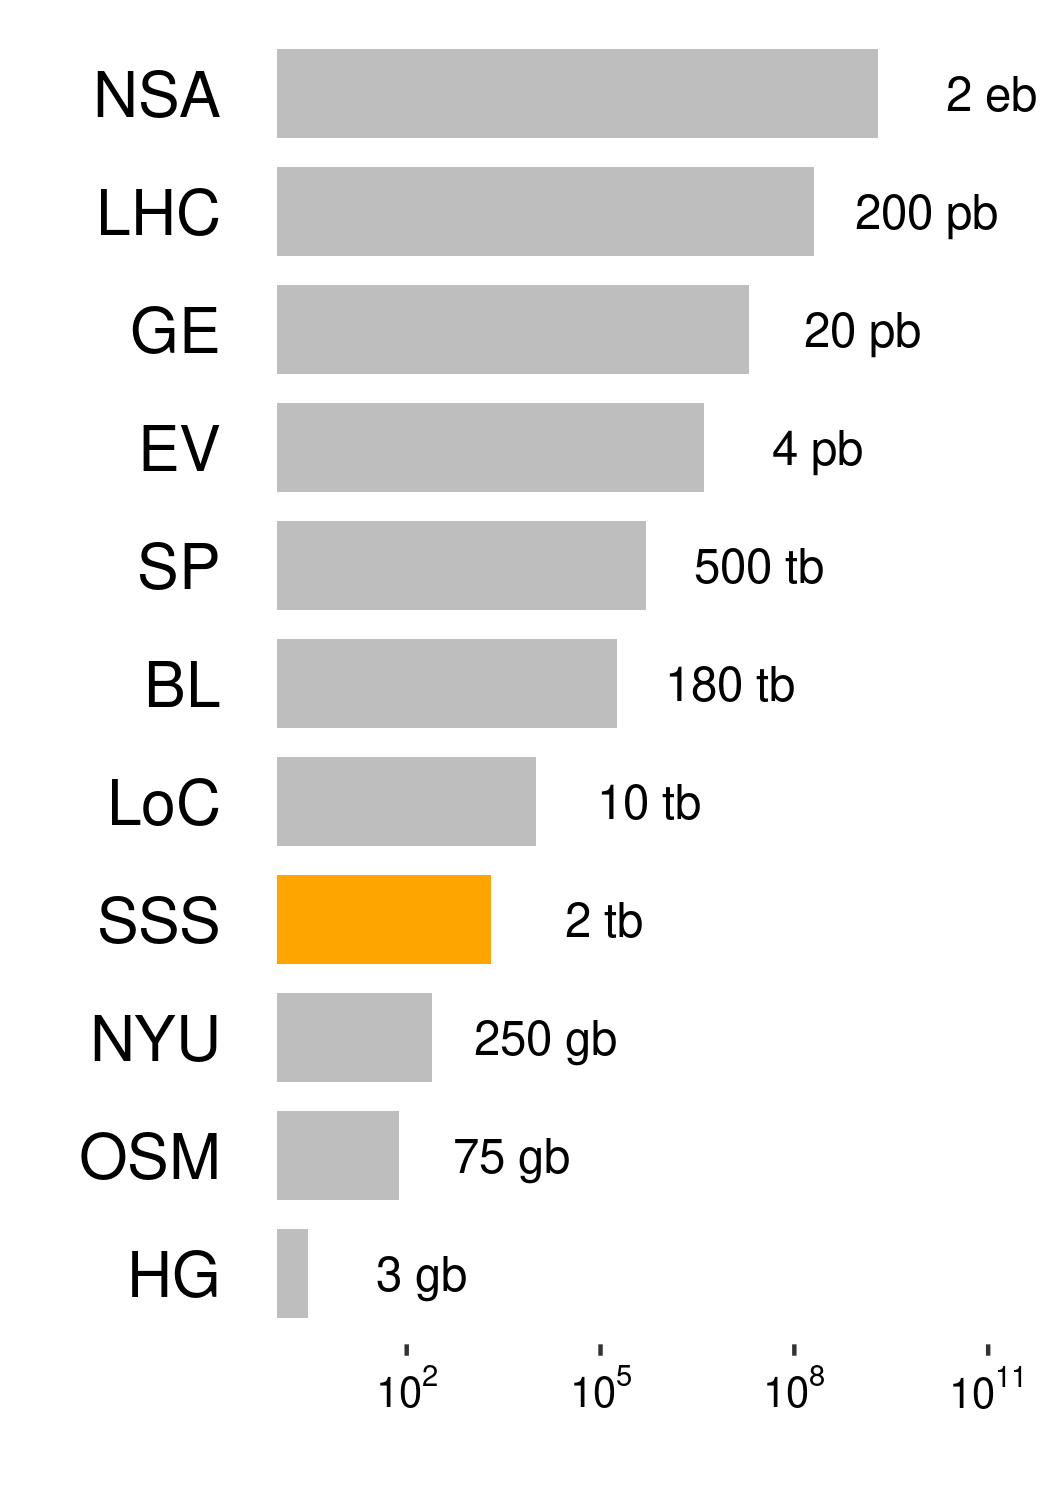
\includegraphics{images/data-size-comparison.png}
  \caption{Comparison of volumes of datasets across various disciplines.}
  \label{figure:toolkit:volume}
\end{marginfigure}

\marginnote[1em]{\fontsize{7}{7}\textit{NSA - National Security Agency, LHC - Large Hadron Collider, GE - Google Earth, EV - Event Horizon project, SP - Spotify music, BL - British Library data store, LoC - Library of Congress, SSS - Smart Street Sensor, NYU - New york city Uber trips 2009-15, OSM - Open Street Map and HG - Human Genome Project}}


%------------------------------------------------------------------------------%

\vspace{1.5em}\noindent\textit{Velocity}\vspace{0.5em}

Velocity is the rate at which the data is collected over time.
It is significant when evaluating big data since some data which may not scale in terms of absolute volume but the speed at which they are received makes them challenging to deal with.
A perfect example is the comparison between data generated by the Large Hadron Collider project by European Council for Nuclear Research and a world wide social network such as Facebook.
Though their total volumes are comparable at 200 petabytes, the data from LHC is generated in concentrated experiments at a rate of 3 petabytes in 5 seconds while Facebook generates the same about in about a day or two.
Since the size of an individual Wi-Fi probe request doesn't vary widely, we define the velocity of this dataset as the number of requests received at a given location at a given location within a given time interval.
Though the precision of the time measured during data collection is in microseconds, the practical data transfer resolution in all the datasets is around 5 minutes.
Hence we measure velocity of out datasets in terms of number of requests every 5 minutes.
Table \ref{table:toolkit:velocity} compares the datasets we collected on Wi-Fi probe requests in terms of their volume.

\begin{table}[h]
  \footnotesize
  \begin{center}
    \begin{tabular}{lcccc}
      \toprule
      Study & Maximum* & Minimum* & Average* & Total** \\
      \midrule
      Pilot Study & 8577 & 188 & 3469 & 3.20 \\
      Main Study & 1362 & 534 & 782 & 0.72 \\
      Smart Street Sensor & 5024 & 6 & 408 & 0.27 \\
      \bottomrule
    \end{tabular}
  \end{center}
  \caption{Comparison of velocity or speed of the datasets of Wi-Fi probe requests.}
  \label{table:toolkit:velocity}
\end{table}

\marginnote{\textit{* Measured/ Estimated for each location in number of requests per 5 minutes. ** Measured/ Estimated for 920 locations in Millions of requests per 5 minutes} }

We observe that locations can receive up to 8500 requests in 5 minutes or can get no request at all depending on the time and how busy it is.
But we can see that on average a national scale project with around 900 locations generates around a million requests every 15 mins. 
Compared to the LHC's 180 billion records or Google's 190 million searches per 5 minutes this seems to be not high speed data.
However, this is much faster compared to traditional data sources such as census or geographical surveys which are updated anywhere between 6 months to 10 years.

To summarise, in terms of velocity, the Wi-Fi probes data can be described as 'Medium' at best. 
The methods dealing with the data should be time sensitive and be able to deal with a continuous stream of data but at the same time need not be real time or need sub-second latency.
Since the Wi-Fi probe requests don't have actual location information the mobile devices, it does not have the similar value in real-time analytics as shown in comparable location or movement based datasets.

%------------------------------------------------------------------------------%

\vspace{1.5em}\noindent\textit{Variety}\vspace{0.5em}

Variety is defined by the amount of variance in the type and characteristics of the data.
Since variety is hard to quantify and compare across disciplines we evaluate the dataset subjectively for the variety present in it.
The data transmitted in a Wi-Fi probe request is defined by the 802.11 Wi-Fi specification \cite{ieee2016} and every probe request has to have a set of mandatory fields for Wi-Fi to work.
This set of fields is the same everywhere across the world and the specification, especially the probe request part, has remained stable over years.
Though there is some variability allowed within the specification, being part of a global standard, the data collected is heavily structured in general.

The first set of variety present in the Wi-Fi probes data set arises from the 'information elements' part of the probe request.
The structure of a probe request is discussed in detail in the data collection chapter and is summarised in Figure ?.
Essentially the information about the capabilities and type of the mobile device is encoded in the information elements part of the probe request and this information is optional and is implemented at the discretion of the manufacturers.
As this information elements are demonstrated to be useful in successfully fingerprinting the mobile devices \cite{vanhoef2016}, mobile devices increasingly don't include any information in them.
Emergence of manufacturers with large market share and narrow set of device models such as Apple and Samsung also reduce further variability in them.
The second set of variety in the dataset arises from the rate at which these probe requests are generated by the mobile devices. 
Unlike devices which generate data on events or at regular intervals, mobile phones generate probe requests at a rate based on various factors.
Though this leads to some challenges in counting footfall from these probe requests the variability exhibited here is neither so large nor so complex that traditional methods could not deal with them.

Comparing with some of the big data encountered in unstructured data collected over web such as social networks or other sensor based methods, the variability here can be considered trivial.
Further when we convert these probe requests in to footfall counts, the variety in the dataset drops almost to zero as it becomes just an ordinal data point varying in geography and time.
Summarising the above, we can confidently say that the Wi-Fi probe request data does not exhibit any `big data' properties in the variety dimension.

%------------------------------------------------------------------------------%

\vspace{1.5em}\noindent\textit{Veracity}\vspace{0.5em}

Veracity is defined as the amount of abnormality present in the data in the form of inaccuracies, biases and noise.
Similar to variety, veracity is hard to quantify hence required a subjective evaluation.
Being sensor collected data, veracity is the dimension where the data exhibits most `big data' properties.


\begin{marginfigure}
  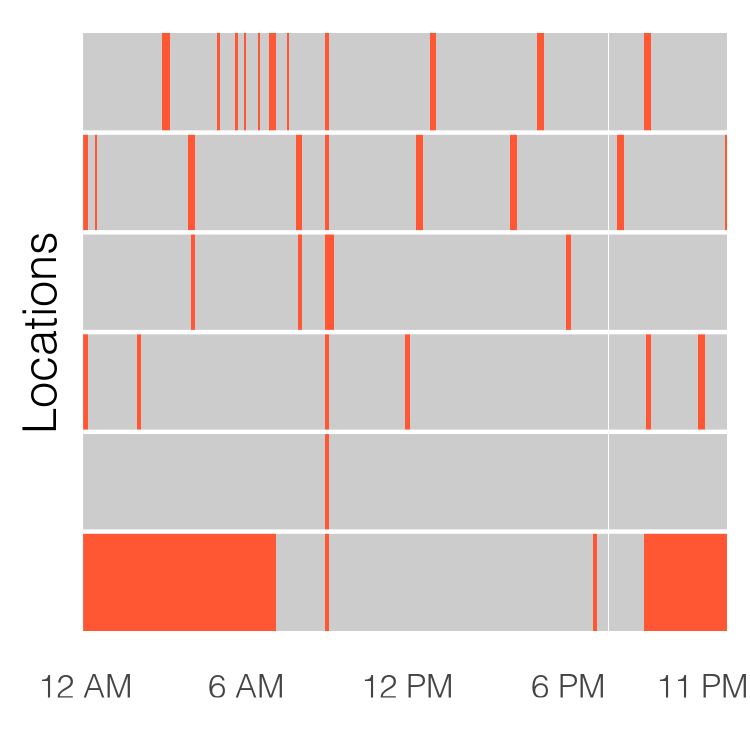
\includegraphics{images/data-veracity-gaps.png}
  \caption{Missing data from five locations at Tottenham Court Road, London on 15 January 2018 demonstrating the veracity of the data.}
  \label{figure:toolkit:veracity:gaps}
\end{marginfigure}

First set of veracity in the dataset arise from the fact that it is collected through sensors located in multiple locations which communicate to the central server using 3G mobile data connectivity.
We know from experience that the sensors are unreliable and fail to send back data regularly due to various reasons.
More over the sensors are installed and uninstalled regularly as partners join and leave the project.
This results in a data stream which is often erratic and incomplete with large gaps in them.
In addition to this the sensors need to be rebooted regularly due to issues or updates leading to small gaps as well.
Since the sensors are part of retail establishments they can be switched on and off regularly in some of them as well.
Figure \ref{figure:toolkit:veracity:gaps} demonstrates the veracity of the data in terms of missing data for a sample of locations in London.
All the above pose immense challenges when we attempt to aggregate the data where we have to estimate and fill these gaps.

There is also a lot of variability in the physical location of the sensors and the area of measurement.
The sensors may report higher or lower count due to their configuration and the context of their location as discussed in chapters pertaining to data cleaning.
This leads to a situation where the accuracy of the data collection varying quite widely across location and times \cite{lugomer2017}.
It is often not clear if the change in the data is due to actual changes at the location or just the change in the configuration of the device.
For example, Opening of a mobile shop next door to the sensor can increase the estimated footfall without any change in actual footfall at the location.

Finally we also have to work within the changing mobile landscape.
Though the Wi-Fi probe requests are standardised by IEEE, the mobile manufacturers have started adopting obfuscation techniques to protect the privacy of the users.
This started with randomisation of MAC addresses, removal of information elements and generally getting more sophisticated with new versions of operating system.
There is also bias in terms of operating system adoption and change in market share between manufacturers.
There is no inherent structure or information on what is changed and how often these changes occur which leads to questions on the continuity of the data over long periods of time.

Summarising from the above, we can confidently conclude that Wi-Fi probe requests dataset shows `Big data' characteristics in terms of its veracity and requires appropriate tools and methods when aggregating, analysing and modelling it.

%------------------------------------------------------------------------------%

\vspace{1.5em}\noindent\textit{Visualisation}\vspace{0.5em}

\begin{figure*}
  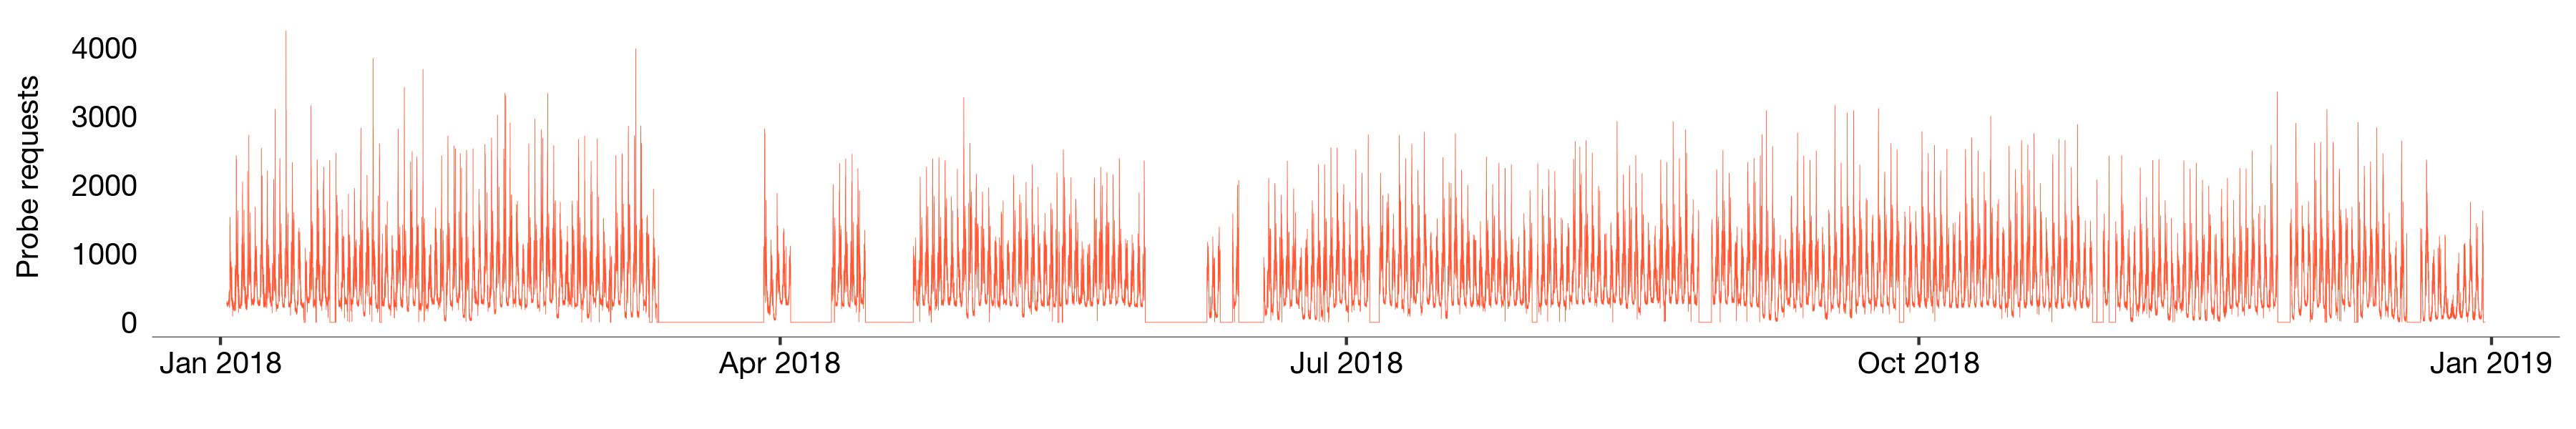
\includegraphics{images/data-visualisation-challenge.png}
  \caption{Number of probe requests collected for every five minute interval at Tottenham Court Road, London on the year 2018 showing the visual complexity of data in the time dimension.}
  \label{figure:toolkit:visualisation}
\end{figure*}

Visualisation is closely related to volume, velocity and variety of the data.
The Wi-Fi data due to its non-trivial volume and velocity, exhibits similar characteristics and challenges in terms of visualisation.
Since there is not much variety in the dataset, when we process the raw data into footfall counts we are left with just the time, location and footfall count for each data point.
Out of these, location and footfall counts are easy to visualise but time exhibits big data properties.
This is primarily due to its granularity at 5 minute intervals and longitudinal nature of the data collection.
The major challenge with Wi-Fi data is to simplify and visualise them in a legible way while showing change in term of time.
The veracity of the data presents challenges in simplifying them and the volume poses challenges in maintaining legibility.
We also have to take the `near real time' aspect of the data into consideration while visualising them.
There is a clear need for always on, interactive, real time dashboards with geographic capabilities in addition to the capabilities of traditional desktop GIS.
There is also need for multiple linked dynamic visualisation platform for separating the scope of the visualisation into manageable units.
Figure \ref{figure:toolkit:visualisation} demonstrates the illegibility of simple visualisations of the data due to granularity, variability and veracity.
We can safely say that the Wi-Fi probe requests dataset is at best `Medium' in the visualisation dimension.

Summarising the above discussion, we can conclude that the datasets collected from Wi-Fi probe requests are at best of 'medium'.
They show the most big data characteristics in terms of their veracity.
In rest of the dimensions the datasets are not truly big data and we need to look at tools and methods appropriate to their size.
The toolkit we devise need to be able to deal with their mid-size volume, velocity and visualisation dimensions and at the same time need to able to deal with the large amount of veracity of in them.
Figure \ref{figure:toolkit:spider} illustrates the summary our discussion.
This leads us to devise a `medium data toolkit' which can be used without incurring the extra cost and complexity introduced by big data tools while be able to handle the data at hand.

\begin{marginfigure}
  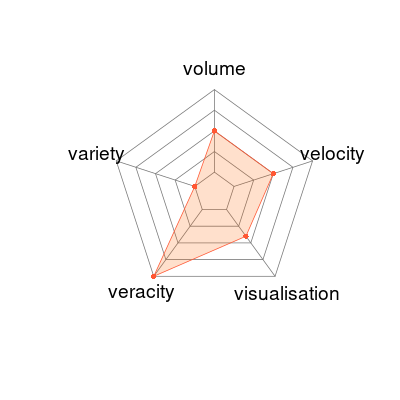
\includegraphics[trim={2.1cm 0 0 0},clip]{images/data-toolkit-spider.png}
  \caption{Big data characteristics of the Wi-Fi probe request datasets in their corresponding dimensions}
  \label{figure:toolkit:spider}
\end{marginfigure}

%------------------------------------------------------------------------------%
% A survey of all tools and methods dealing with big data.
%------------------------------------------------------------------------------%

\subsection{A Survey of Methods and Tools}

Having classified the Wi-Fi probes dataset as a `Medium' sized data, in this section, we survey the tools and methods available at various stages of the data processing and management process - data collection, storage and retrieval, processing and analysis, visualisation.
We first survey the tools available in each stage and specifically look at their suitability for Wi-Fi probe request datasets in terms of the following characteristics,

\begin{itemize}
  \setlength{\itemindent}{1em}
  \itemsep-0.25em
  \item \textit{Performance} - How much data can be processed in a given time?
  \item \textit{Flexibility} - How easy it is to change the scale and scope?
  \item \textit{Complexity} - How many components or parts are involved?
  \item \textit{Cost} - How much money or infrastructure do they require?
\end{itemize}

We then discuss the principles of UNIX philosophy and how it helps in solving similar sized problems in computer science. Finally we pick and connect the tools to devise our toolkit which is best suited for out Wi-Fi probe request dataset.

%------------------------------------------------------------------------------%

\vspace{1.5em}\noindent\textit{Collection}\vspace{0.5em}

We discussed various technologies used in collecting passive data on ambient population and pedestrian movement in the literature search.
In this section we look at tools and methods used to collect Wi-Fi based data passively.
The primary considerations for evaluating data collection strategy are the scale of the infrastructure, expertise and effort required to implement it and cost involved.

There have been numerous sensors, tools and associated software platforms made available for data collection under the umbrella of `internet of things'.
We start by looking at different approaches in the Wi-Fi data collection tools and try to reason the most appropriate solution for our research.
On one end there are low level and low cost bespoke solutions which require lot of effort to implement and maintain.
On the other end there are turn key solutions which doesn't require lesser effort but costs considerably more.
The key is finding a balance between both while satisfying the requirements of the project.
Since the Wi-Fi data is medium sized in terms of volume and velocity, we can deal with solutions with less than optimal scalability but since the data is 'big' in terms of veracity the toolkit has to give us most flexibility. 
Essentially, we are looking for a data collection methodology which prioritises flexibility and cost while performing moderately in terms of scalability and complexity as illustrated in Figure \ref{figure:toolkit:collection}.


\begin{table}[h]
  \footnotesize
  \begin{center}
    \begin{tabular}{lp{5cm}}
      \toprule
      Type of solution & Examples\\
      \midrule
      Bespoke & Micro-controllers with Wi-Fi modules e.g. Audrino + ESP8266\\
      Turn-key & End to end commercial services e.g. Blix, Euclid, Pygmalios etc.\\ 
      \textbf{Ideal} & \textbf{General purpose hardware e.g. Raspberry Pi, Repurposed mobile devices - Tablets, Phones etc.}\\
      \bottomrule
    \end{tabular}
  \end{center}
  \caption{Examples of different types of Wi-Fi based data collection solutions.}
  \label{table:toolkit:collection}
\end{table}

In terms of hardware, an example of a highly customised solution would be a micro-controller, such as Audrino, coupled with dedicated Wi-Fi module and programmed with custom software to collect the exact data needed.
Designing and implementing of such system is time consuming, cumbersome and usually involves significant cost but it can also be highly flexible, efficient and cheap to deploy.
On the other end of this spectrum, we have end-to-end solutions such as Blix, Walkbase, Ecuclid, Retail next, pygmalios etc. where the data is collected through multiple sensors and sources and syndicated into a clean footfall information by a third party service provider.
These platforms for footfall data collection and analysis have the advantage of being quick and easy to develop and deploy while they can also be highly inflexible for changes and turn out to be costly when scaled up.
A middle ground here is to use a general purpose hardware such as single board computers or repurposed mobile devices, augment them with additional hardware modules and use general purpose scripting languages to write software for them.
This way we avoid low level hardware or software design and implementation while maintaining good amount of flexibility.
Table \ref{table:toolkit:collection} shows some examples of such systems while highlighting an ideal system.

\begin{marginfigure}
  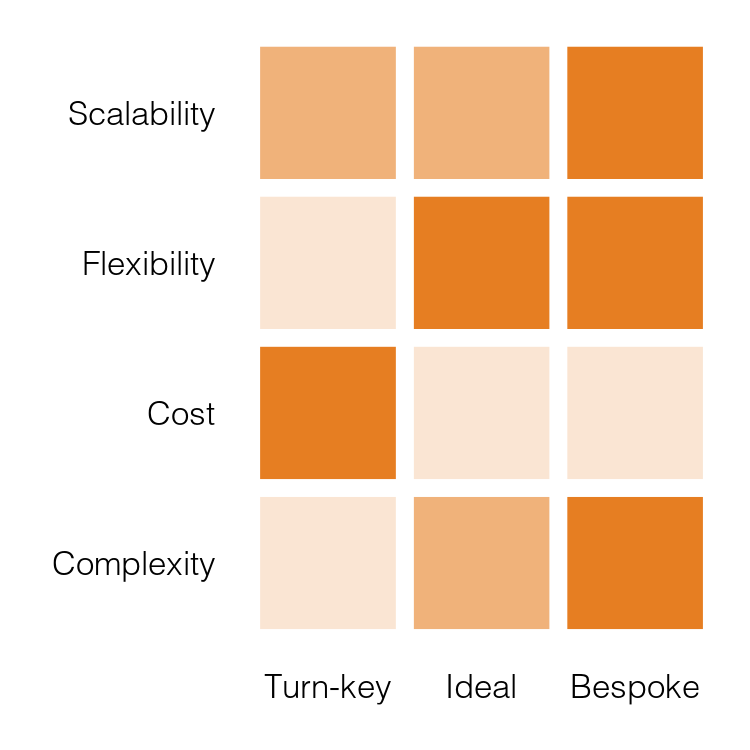
\includegraphics[trim={0.2cm 0 0 0},clip]{images/data-toolkit-collection.png}
  \caption{Characteristics of types of Wi-Fi data collection tools at each end of the spectrum compared to an ideal candidate  }
  \label{figure:toolkit:collection}
\end{marginfigure}
\marginnote[0.1cm]{\textit{(Darker colors show higher score)}}

The Smart Street Sensor project uses its own proprietary sensor system designed and instrumented by the data partner.
The design and implementation decisions were made with the commercial application in mind and is not entirely relevant to our discussion in the context of our research.
For the research conducted with the data, it is necessary to understand the data collection process and make sure it aligns and integrates with the rest of the toolkit.
As discussed in the data collection chapter, the methodology used in the smart street sensor project satisfies our requirements.
The toolkit we designed to collect other datasets are in-part inspired by this methodology or a modified version to include more flexibility.
The toolkit consists of Raspberry Pi, Linux, tcpdump or tshark \cite{wireshark2} and nodejs.
Raspberry Pi and the Linux OS provides a general purpose base system and hence the flexibility.
On top of this we built our data collection system by assembling open source and free network analysis tools such as tcpdump and tshark along with other tools providing functions such as scheduling, personal data obfuscation and data transmission with scripting languages like nodejs and bash.

%------------------------------------------------------------------------------%

\vspace{1.5em}\noindent\textit{Storage}\vspace{0.5em}

Data storage technology is one of the most diverse landscape in terms of both methods and tools available.
It has been constantly in research and development since the beginning of computing and is one of the fastest changing landscapes with the advent of big data paradigm.
A comprehensive review of storage solution warrants a chapter in itself so we restrict our survey to an outline of most significant approaches and corresponding systems and tools.

At one end of the spectrum is one of the most underappreciated for of data storage - File systems.
Though they seem like a low level interface for storing data, file systems have their advantages as well.
When the data is not complex or inter-related, flat text files in file systems could be the fastest way to store, search and retrieve data.
Since operating systems are usually optimised to manage storage media through file systems, they involve no additional overhead and are extremely reliable.
The hierarchical file systems use in most of the operating systems act as an index with hierarchical data.
The major disadvantage of file systems is that they are not useful for managing data with any kind of complexity.
This is the primary reason why database management systems are developed on top of file systems.

Database systems can be broadly divided into relational and document based.
The relational databases are optimised to deal with relational data and usually enforce strict structure for the data
In general they can handle large number of rows and are designed to scale vertically.
Most relational database systems try to guarantee ACID \sidenote[][-7cm]{Atomicity, Consistency, Isolation and Durability are properties which make sure that the data in the database is valid even during failures.} compliance and hence used in critical systems such as financial operations, sales etc \cite[-5cm]{Haerder1983}.
The document based databases are optimised to deal with unstructured data and can doesn't need a strictly defined scheme.
In general they can handle large number of columns and are designed to be distributed and scaled horizontally.
Being distributed, most document based databases try to pick a focus and compromise on others as specified in CAP theorem \sidenote[][-3cm]{Brewer's theorem or CAP theorem states that it is impossible to simultaneously guarantee consistency, availability and partition tolerance in a distributed data store.}.
There a numerous databases systems which prioritise different things and the right solution depends on the properties of the data and the requirements of the project.

Since the publication of the paper on `Google file system' by google \cite{sanjay2003}.
There have been significant effort in designing and building 'big data' file storage systems which can large data in the range of petabytes.
These systems are designed to be distributed and optimised for high throughput for queries on them.
Hadoop Distributed File System (HDFS) is one such file system which is also the most widely adopted.
There are numerous cloud based, third-party solutions built with these file systems making them easy to use.
There are also numerous tools, libraries and frameworks which emulate the features of database systems on these distributed file systems making them easier to use further.
The primary advantage of these systems is the sheer scalability they provide when it comes to data volume.
The primary disadvantage is the associated overheads in terms of cost and time incurred in learning, designing and implementing them.
Unless the project is sufficiently large, the advantages gained usually do not justify the overheads introduced.
Table \ref{table:toolkit:storage} summarises the above discussion along with relevant examples.

\begin{table}[h]
  \footnotesize
  \begin{center}
    \begin{tabular}{lcp{2cm}p{4.5cm}}
      \toprule
      Approach & Data size & Examples & Comments\\
      \midrule
        File system &
          \textless{} 10 TB &
          ext, ntfs, zfs, btrfs &
          Simple and efficient. Best for hierarchical data. Cannot handle complex connected data.\\
        \addlinespace[0.2cm]
        Relational DB &
          \textless{} 5 TB &
          MySQL, PostgreSQL&
          Handles structured and relational data. Optimised for large amount of rows and tries to guarantee validity.\\
        \addlinespace[0.2cm]
        Document DB &
          \textless 10 TB &
          MongoDB, Cassandra&
          Handles unstructured data. Optimised for large number of fields and distribution to multiple clusters. Tries to focus on any two guarantees of the Brewer's theorem.\\
        \addlinespace[0.2cm]
        Distributed FS &
          \textgreater{} 10 TB &
          HDFS, Ceph, GFS &
          Optimised for really large datasets which need to be distributed over multiple nodes.\\
        \addlinespace[0.2cm]
        Cloud Storage &
          \textgreater{} 10 TB &
          AWS, Azure, SWIFT &
          Implements distributed file systems on the cloud. Has more reliability and scalability than local implementations.\\
        \addlinespace[0.2cm]
        Data Warehouse &
          \textgreater{} 10 TB &
          Hive, Hbase, Impala, Presto&
          Interfaces built on top of distributed file systems to emulate capabilities of relational databases on them.\\
      \bottomrule
    \end{tabular}
  \end{center}
  \caption{Various data storage approaches and their characteristics.}
  \label{table:toolkit:storage}
\end{table}

We saw that the Wi-Fi probe request datasets are `Medium' sized hence we can safely eliminate distributed file systems for storing them.
Though the smart street Sensor project uses Azure Blob Storage, when the data is downloaded to the local servers at the university, we can just store them in the file system because of their size (2TB approx.) and the hierarchical nature.
The folder structure of - year/month/day/location/interval/ with individual text file, enable us to query the data for any given location at any interval nearly instantaneously without any further database operations.
When this raw data is processed into 5 minute counts, we require more relational queries.
For this purpose a relational database is sufficient as volume is quite small (25GB approx.).
We chose PostgreSQL because of the PostGIS extension which gives us flexibility in handling geographic data.

%------------------------------------------------------------------------------%

\vspace{1.5em}\noindent\textit{Processing}\vspace{0.5em}

\begin{marginfigure}
  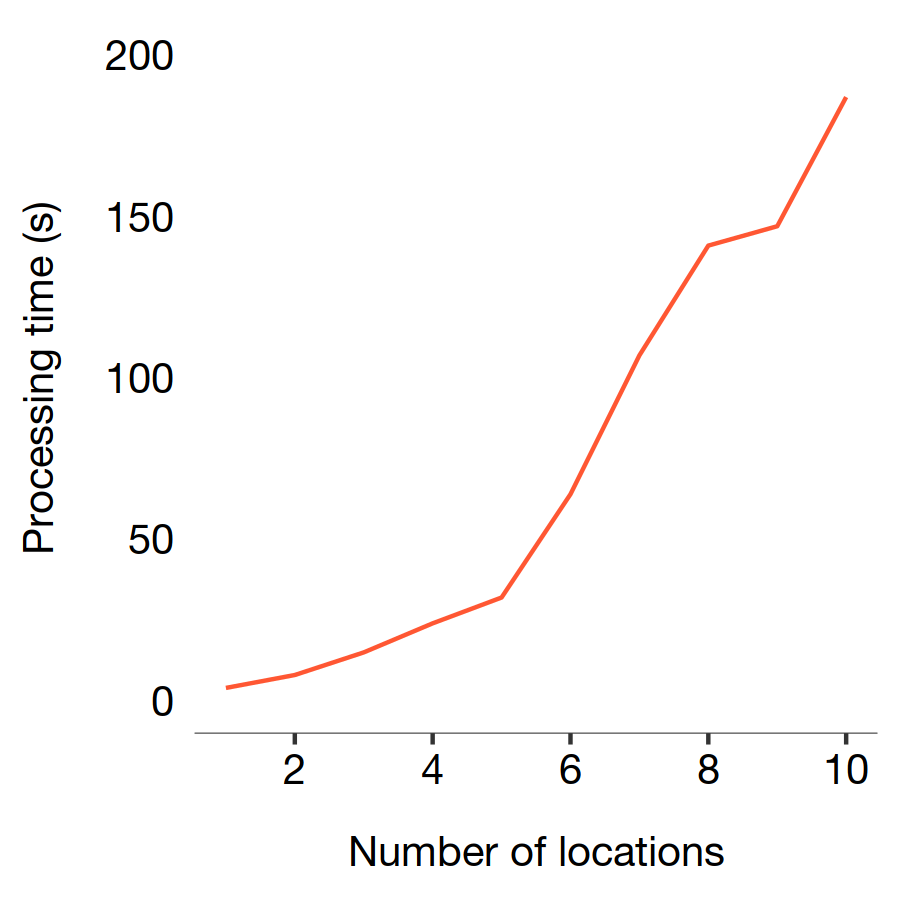
\includegraphics[trim={0 0 0 0},clip]{images/processing-time-old.png}
  \caption{Exponential increase in the processing time when using traditional methods.}
  \label{figure:toolkit:time:old}
\end{marginfigure}

\marginnote[1em]{\fontsize{7}{7}\textit{The processing involves parsing JSON data received for a single day at each location and aggregating them as number of probes requests received in every five minute intervals.}}

We saw that the data is medium in terms of volume and velocity and shows big data properties in terms of veracity.
Hence we require tools which are capable of dealing with the veracity of the data while being able to manage the volume and velocity.
The traditional approach to deal with such dataset is to load it into a general purpose analysis tool such as R or a GIS packages and process it.
The size of the dataset and the lack of meaningful complexity of geography element in the data eliminates the use of GIS packages.
Scripting languages such as R and Python can deal with the dataset and its requirements but the time taken to do so increases exponentially with the size of the data as the size of objects in memory increases.
Figure \ref{figure:toolkit:time:old} illustrates the increase in processing time with respect to number of location for a simple exercise where a day's worth of raw data is parsed and aggregated into number of probe requests per 5 minute intervals 
(The code used to produce these benchmarks are detailed at Section \ref{appendix:benchmark}).
This becomes prohibitively expensive as the number of locations and complexity of the processing increases.
Though this can be improved with more efficient coding practices, the margin of improvement is quite limited hence creating the need for better techniques.
It is important to note that data processing is done in two stages - the first stage where the raw Wi-Fi probe requests are filtered, cleaned and aggregated into footfall counts and second stage where the footfall counts are in turn analysed to produce reports and visualisations.
The traditional methods are sufficient for the second stage of the processing and the first stage is the one which requires a better solution.

On the other end we have big data analysis tools which are built for dealing with extremely large amount of data.
Since the publication of the paper on MapReduce, there have been immense developments in the Big data analysis landscape.
There numerous distributed programming tools to use the data stored within a distributed storage system each focussing on specific type of data and analysis.
A concise, non-comprehensive list of types of data or specialities and corresponding big data tools is shown in Table \ref{table:toolkit:processing}.

\begin{table}[h]
  \footnotesize
  \begin{center}
    \begin{tabular}{lp{3cm}}
      \toprule
      Tools & Speciality\\
      \midrule
        General purpose & MapReduce, Spark\\
        Real-time streams & Flink, Pulsar\\
        Events or messages data & Storm, Kafka, Flume\\
        Networked or graph data & Tinkerpop, Corona \\
        Scheduling & Oozie, Falcon, Azkaban\\
        Turn-key platforms & SpringXD, Cask Data\\
      \bottomrule
    \end{tabular}
  \end{center}
  \caption{Various types of big data processing tools and corresponding examples.}
  \label{table:toolkit:processing}
\end{table}

We can rule out the necessity of the above big data tools since our dataset is neither big enough nor fast enough.
The dataset does not have any specialised structure such as graph or network but just a very minimal component of geography to it.
Using any of specialised big data tools is just going to introduce immense overheads without any added benefits.
We need something in-between the above two approaches where we is sufficiently fast and flexible for our datasets.

This is where we come across the possibility of using standard Unix tools along with connecting them to create a processing pipeline.
In some cases, a data processing pipeline made using command line Unix tools have been demonstrated to be 230 times faster than using big data toolkits \cite[-2cm]{adam2014}.
The command line tools were developed as parts of Unix operating system for processing text. 
They are developed in line with the Unix philosophy which focuses on modular and minimal software development. 
The core tenants of the Unix philosophy has been summarised by Doug McIlroy as below,\cite{mcilroy1978},

\begin{enumerate}[rightmargin=1cm]
  \setlength{\itemindent}{2em}
  \itemsep-0.25em
	\item Make each program do one thing well. To do a new job, build afresh rather than complicate old programs by adding new "features".
	\item Expect the output of every program to become the input to another, as yet unknown, program. Don't clutter output with extraneous information. Avoid stringently columnar or binary input formats. Don't insist on interactive input.
	\item Design and build software, even operating systems, to be tried early, ideally within weeks. Don't hesitate to throw away the clumsy parts and rebuild them.
	\item Use tools in preference to unskilled help to lighten a programming task, even if you have to detour to build the tools and expect to throw some of them out after you've finished using them.
\end{enumerate}

\begin{marginfigure}
  \forcerectofloat
  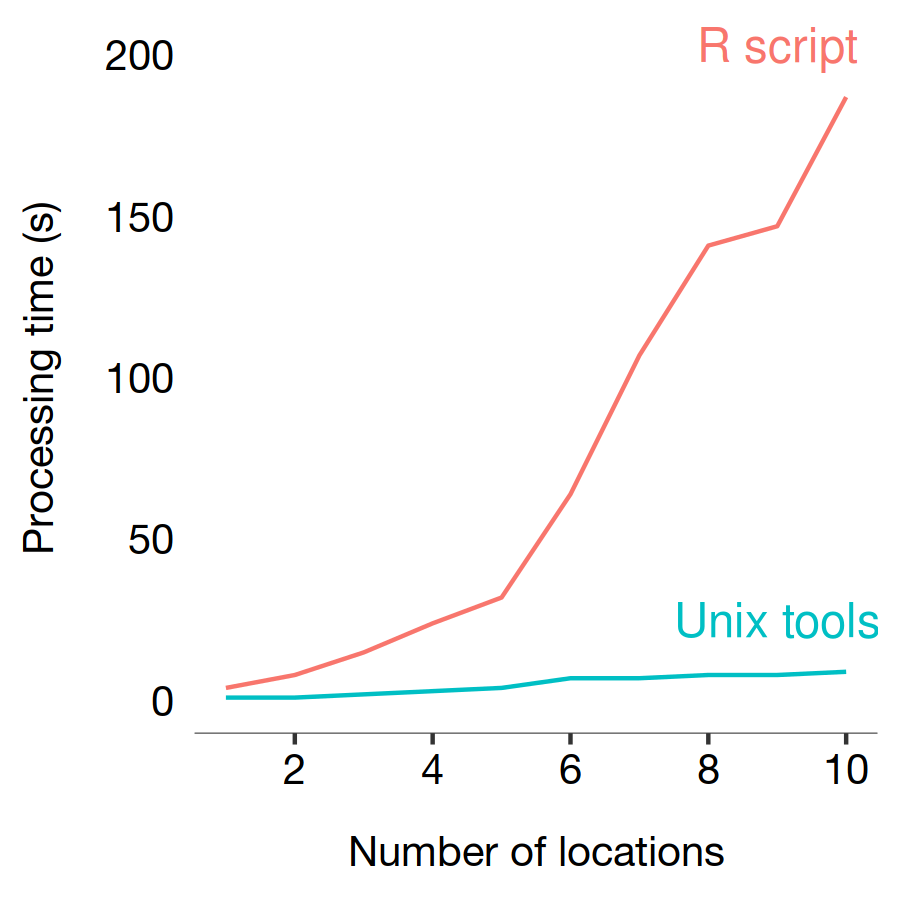
\includegraphics[trim={0 0 0 0},clip]{images/processing-times-r.png}
  \caption{The increase in processing time with the Unix pipeline is linear thus improves the scalability compared to R based processing}
  \label{figure:toolkit:time:new}
\end{marginfigure}

These principles along with the `pipe' operator gives us necessary tools to build more complex tools.
We can replace most of the libraries we used in the R implementation of our processing with a corresponding command line tools and connect them together with a text interface to achieve similar pipeline.
The first advantage of such design is that it is much more efficient than a monolith design.
These tools being actively developed for since their invention are compiled as native binaries and are usually extremely optimised resulting in a much faster pipeline.
Because of the design of the pipe operator, the individual parts of the pipeline are executed in parallel as chunks of data are passed through them thus avoiding the need to load entire datasets into memory which results in an exponential increase processing time with the size of the data.
Being modular, we can even introduce process level parallelism to parts of the pipeline without any major change in the overall design.
Finally the modular structure also gives us the advantage of using the best tool for any part of the pipeline.

\begin{table}[h]
  \footnotesize
  \begin{center}
    \begin{tabular}{p{4cm}p{3cm}p{3cm}}
      \toprule
      Tools & R Library & Unix tool(s)\\
      \midrule
        Move data to and from Azure blog storage, SQL server and Postgres & AzureR, odbc , RPostgreSQL & azcopy, mssql, psql\\
				Convert data from JSON format to CSV & jsonlite & jq\\
        \addlinespace[0.2cm]
				Encrypt raw data for secure storage & Rcrypt & gnupg\\
        \addlinespace[0.2cm]
				Anonymise personal data into cryptographic hash & digest & openssl\\
        \addlinespace[0.2cm]
				Transform and manipulate tabular data& dplyr & find, cat, cut, grep, sed, awk, sort, uniq, column, paste, join\\
        \addlinespace[0.2cm]
				Impute missing value using time series analysis & imputeTS & Rscript\\
        \addlinespace[0.2cm]
				Visualise the results into maps and charts & ggplot2 & Rscript\\
        \addlinespace[0.2cm]
        Create and manipulate geographic data & sf, rgdal & postgis, gdal\\
      \bottomrule
    \end{tabular}
  \end{center}
  \caption{Tasks in the processing pipeline, corresponding R libraries and equivalent Unix tools}
  \label{table:toolkit:tools}
\end{table}

\begin{marginfigure}[2cm]
  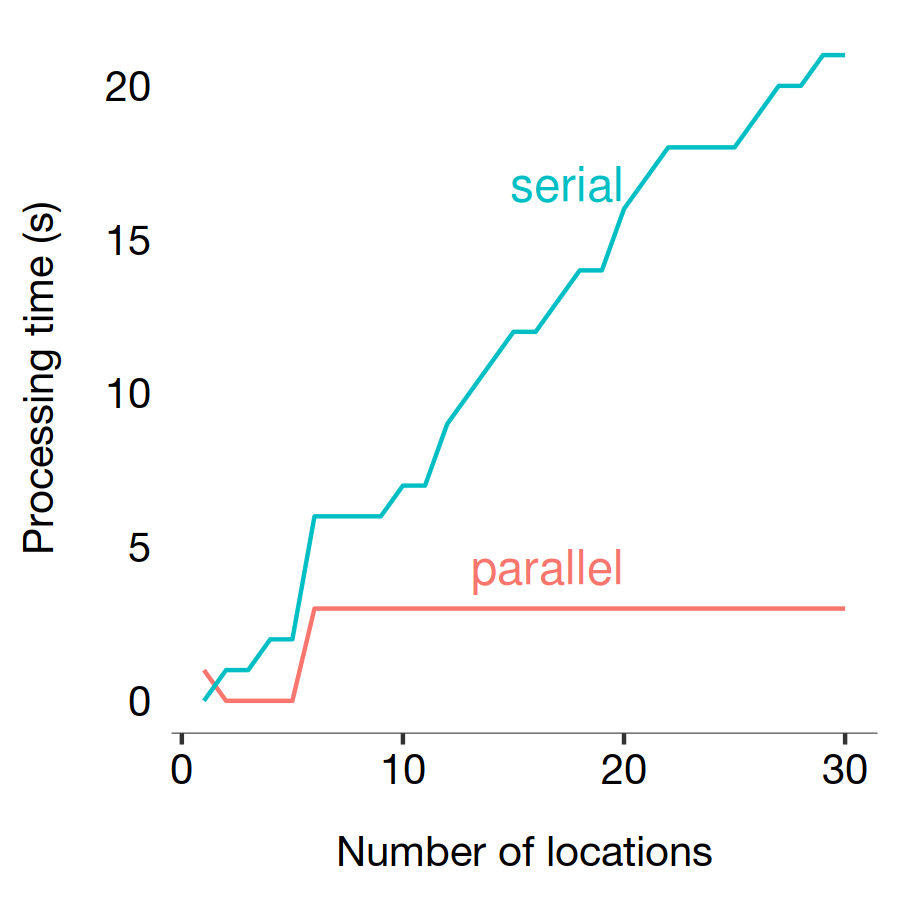
\includegraphics[trim={0 0 0 0},clip]{images/processing-times-parallel.png}
  \caption{The scalability of the processing pipeline could be further improved with parallelising it.}
  \label{figure:toolkit:time:parallel}
\end{marginfigure}

All of the gives us an extremely minimal and efficient toolkit to process the raw Wi-Fi probes data into counts in a scalable way.
Figure \ref{figure:toolkit:time:new} compares the processing times of such Unix toolkit with the traditional R based toolkit as the data size increases.
We can see that Unix toolkit performs extremely well and the performance gains are significant as the size of the data increases.
For example, to process data for 25 locations, R based toolkit takes around 20 minutes while the Unix toolkit gets it done in 20 seconds 
(The code used to produce these benchmarks are detailed at Section \ref{appendix:benchmark}).
Table \ref{table:toolkit:tools} shows the activities in our pipeline and corresponding libraries in the traditional R workflow along with the equivalent Unix tools.
It is important to note that tools for doing specialised actions such as statistical analysis, machine learning and time-series analysis are built on top of scripting languages such as R and Python.

These can be embedded into our Unix pipeline as scripts running in corresponding front-ends such as Rscript or python.
This toolkit can be further accelerated by parallelising parts of the pipeline using gnu-parallel \cite{tange2018}.
For example, the previous example pipeline can be parallelised by spawning a pipeline for each location this reduces the processing time for a set of 25 locations from 18 seconds to 3 seconds.
This done by utilising every processor cores available in the CPU.
Figure \ref{figure:toolkit:time:parallel} compares the processing times of the Unix toolkit with a parallelised implementation (The code used to produce these benchmarks are detailed at Section \ref{appendix:benchmark}).
Finally all the Unix tools discussed in this toolkit are open source and free software which has almost no cost in terms of resources.
Since these tools are part of the POSIX specification \cite{walli1995} for operating systems, the expertise in their design and use are transferable to and from other disciplines thus reducing researcher time learning and using these tools.


%------------------------------------------------------------------------------%

\vspace{1.5em}\noindent\textit{Visualisation}\vspace{0.5em}

In the last section we saw that the visualisation dimension of the data shows some level of complexity.
The primary source of this complexity arises from the longitudinal nature of the data and the noise due to granularity of the data.
For the processed dataset, traditional visualisation and mapping libraries with R is sufficient while the visualisation of raw data across long time periods for either for exploratory analysis or for communication needs some form of interactivity or simplification to be able to legible.
Data driven documents (D3) \cite{stanford2011} and Dimensional charting (DC) provides us with both of these requirements.
Both of these tools can accept text based input and can fit with other Unix tools discussed earlier.
In case of binary file output such as images or documents, they could be directed to the file system and then read into other programs.

%------------------------------------------------------------------------------%
% Final summary and conclusions
%------------------------------------------------------------------------------%

\subsection{The Bespoke `Medium data toolkit'}

In this chapter we saw how the advent of internet and internet enabled devices has lead to significant increase in the amount of data generated and collected across disciplines. 
This data deluge and improvements in the capabilities of computing hardware has fuelled an explosion of research and development in tools and methods to deal with these `Big data'.
Though these big data tools promise huge improvements in processing capabilities, when used under wrong circumstances they can lead to unwanted overheads and costs.
Thus we need a framework to examine and understand the scale of the data that is being used so that we use the right tools for the right purposes and the 5Vs of `Big data' - Volume, Velocity, Veracity, Variety and Visualisation provides us with such frame work.
Every dimension of big data poses unique set of challenges and we need make right decisions in choosing specialised tools and methods to overcome them.

We then closely examined the Wi-Fi probes data we collected with this framework and found that the data, though posed significant challenges with traditional data processing techniques, do not exhibit `big data' properties in all its dimensions. 
Only veracity of the data was found to have any meaningful big data properties, while volume and velocity was found to be 'medium' at best. 
The datasets lacked any variety and posed minimal challenge in the visualisation dimension because of it high temporal granularity.
Thus we arrived at the requirements for a bespoke `medium data toolkit' which is able to deal with these challenges.

\begin{figure}
  
\includegraphics{images/toolkit.png}
  \caption{Outline of the `Medium data toolkit' devised to collect, process, visualise and manage the Wi-Fi probe requests data}
  \label{figure:toolkit}
\end{figure}

We undertook a brief survey of tools available for collecting, storing, processing and visualising the Wi-Fi probe request data and with the understanding of the data from the previous analysis chose the ones which are perfect for the datasets.
For collecting Wi-Fi probes data in a scalable way, we chose a general purpose single board computers such as Raspberry-Pi along with open source tools such as tcpdump and tshark in a Linux environment.
For data storage we narrowed in on using just the file system for the raw data and relational database management system for the processed counts.
To process the raw data we chose to devise a processing pipeline using an assortment of standard Unix command line tools linked together using a shell scripting language and parallelised at the process level with gnu-parallel.
We also demonstrated that this processing pipeline can be 400 times faster than the using a monolithic pipeline even with a small sample of locations.
For visualisation we chose D3 and DC as the solution for communicating time information legibly.
Finally we arrive a `medium data toolkit', illustrated in Figure \ref{figure:toolkit}, which is best suited for the Wi-Fi probes dataset which we employ to process and examine the data further.


\cleardoublepage
\section{Device fingerprinting}

In the past decade, Wi-Fi has emerged as one of the most commonly used technologies in providing high speed internet access to mobile devices such as smartphones, tablets and laptops in public and private spaces \citep{torrens2008}.
This has resulted in multiple Wi-Fi networks being available at almost every location in dense urban environments.
Traversing through this overlapping mesh of Wi-Fi networks, modern mobile devices with Wi-Fi network interfaces regularly broadcast a special type of signal known as `Probe Requests' in order to discover the Wi-Fi networks available to them.
This helps these devices to connect and switch between the Wi-Fi networks seamlessly.

Probe requests are low level signals standardised by IEEE 802.
1 specification \citep{ieee2016} for service discovery, and are implemented in any Wi-Fi capable device irrespective of the manufacturer or the model.
This ubiquity and standardisation makes them an excellent source of open, passive, continuous, and wireless data generated by Wi-Fi capable devices present at any given time and location.
Considering the unprecedented levels of mobile device ownership in recent years, we can, in turn use this data to understand the population distribution in highly dynamic urban environments with high spatial and temporal granularity \citep{freud2015, konto2017}.
While a Wi-Fi based method to collect data offers us various advantages such as, easy scalability and efficiency in terms of cost and time, it also introduces few systematic biases and uncertainties in the collected data along with the serious risk of infringing on the privacy of the mobile users.
In this section, using the set of probe requests and manual counts collected at various high street locations across London, we demonstrate that pedestrian footfall at these locations can be estimated with considerable precision and accuracy while protecting the privacy of the pedestrians.

Unlike GPS, the location of the Wi-Fi enabled mobile device cannot be directly inferred from Wi-Fi, however there are reliable methods to triangulate the location of mobile devices from the locations of known access points (AP) and the signal strength reported by them \citep{he2003, moore2004, lamarca2005}.
This can overcome the usual shortcoming of GPS, which struggles for precision and accuracy in indoor and densely built environments \citep{zarim2006, kawaguchi2009, xi2010}.
Utilising this, we can easily and quickly estimate trajectories of the mobile devices \citep{musa2012} which can be used similarly to the GPS trajectories to understand individual travel patterns \citep{rekimoto2007, sap2015}, crowd behaviour \citep{abedi2013, mowafi2013}, vehicular \citep{lu2010} and pedestrian movement \citep{xu2013, fukuzaki2014, wang2016}.
Such data can also be used in transportation planning and management to estimate travel time \citep{musa2011} and real time traffic monitoring \citep{abbott2013}.
Using techniques demonstrated by \citep{franklin2006} and \citep{pang2007}, along with information present in the probe requests, one can even model interactions between the users \citep{cheng2012, barbera2013, cunche2014} such as predicting which of them are most likely to meet again \citep{cunche2012}.
Using the semantic information present in these probe requests it even is possible to understand the nature of population at a large scale \citep{di2016}
.

Although extensive research has been carried out on this subject with feasible and favorable results, in recent years, one of the major challenges faced in such attempts has been the increasing attempt by mobile phone manufacturers to protect their users’ privacy by anonymising the globally identifiable portion of the probe requests \citep{greenstein2008}.
Various methods have been devised to overcome this anonymisation process such as estimating the device model information from a known dataset of manufacturers and device behaviours \citep{martin2016}; Scrambler attack using a small part of the physical layer specification for Wi-Fi \citep{vo2016, bloessl2015}; and timing attack where the packet sequence information along with information elements present in the probe request frame is used \citep{matte2016, cheng2016}. A combination of these methodologies has been proven to produce de-anonymised globally unique device information \citep{vanhoef2016, martin2017}. These approaches usually result in serious risk of breach of privacy of the users of the mobile devices by revealing their identifiable personal information.

There is a clear gap in the research for exploring methodologies for estimating the number of unique mobile devices from a set of anonymised probe requests, without the need to reveal their original device information.
Such a technique has various applications such as uncovering the urban wireless landscape \citep{rose2010}, revealing human activity at large scales \citep{qin2013}, estimating pedestrian numbers in crowds \citep{schauer2014, fukuzaki2015}, and even counting people in hyper local scales such as queues \citep{wang2013}.
With enough infrastructure to collect such information we can even aim to generate a real-time census of the city \citep{konto2017}.
With this background, we set out to devise and implement a methodology to reliably estimate human activity such as pedestrian footfall from Wi-Fi probe requests without risking a breach of privacy of the users involved. 

\vspace{1.5em}\noindent\textit{Methodology}\vspace{0.5em}

The primary aim of this research was to enable us to collect a series of probe requests and process them into a usable pedestrian footfall count.
We did this by using a Wi-Fi receiver to collect probe requests broadcast by mobile devices, filtering out the background noise, and aggregating them based on the device that generated them.
In this section, we examine the characteristics of probe requests in detail, devise a methodology to collect these probe requests in public areas, examine the systemic biases and uncertainties in the data collection method, and devise data processing methods to overcome these challenges.
Finally, we compare the processed footfall counts to the ground truth recorded by primary surveys.

Probe requests are a special type of management packet broadcast by Wi-Fi enabled devices as part of their various functions such as scanning for available APs and quick geolocation by triangulation based known APs, etc.
These are broadcast by all Wi-Fi enabled devices regardless of the manufacturer, type or model of the devices, although there is some variation in the frequency and the content of the information transmitted through them.
In some cases, such as Android devices, these are broadcast even when the Wi-Fi functionality has been turned off by the user so that the device can immediately connect to networks when the functionality is switched back on.
Since some devices even use the probe requests as a less accurate form of localisation, they continuously send probe requests when Wi-Fi has been switched off.
Thus, these signals can be used to reliably identify the presence of Wi-Fi enabled mobile devices.
Being a first step of connection initiated by the mobile device, these packets have information regarding the characteristics of the mobile device itself.
Some of the key information we can infer from these requests are,

\begin{enumerate} 
\item \textbf{Media Access Control (MAC) address} which is a name identifying the wireless hardware of the mobile device, 
\item \textbf{Sequence number} of the request for the mobile device to keep track of the responses, 
\item \textbf{Time stamp} at which the request was received by the AP, 
\item Total \textbf{length} of the request in number of bits, and 
\item The \textbf{strength of the signal} received by the mobile device.
\end{enumerate}

The MAC address is the primary identifier for the mobile device and has two parts.
The first part is the Organisationally Unique Identifier (OUI) which provides information about the manufacturer of the device and the second part is the identifier for the device.
In modern devices, to protect users' privacy, the second part of the MAC address can also be randomised and hence may not be unique to devices.
When the MAC address is randomised, it is marked as such by setting a specific bit in the probe request packet as 1.
Although sequence number of the packet is strictly unique to a mobile device, we hypothesize that we can use them to estimate the number of unique devices as demonstrated by \citep{vanhoef2016}; where optional information present in the probe requests - Information Elements (IE) along with the sequence numbers, have been used to fingerprint the devices.
This approach has become increasingly difficult as mobile phone manufacturers have severely limited the IEs present in the probe requests thus leading us to explore methods which use only the sequence numbers.
This also affects the established commercial solutions using Wi-Fi probe requests such as Blix, Walkbase, Euclid Analytics, RetailNext etc.
There has been another solution proposed by \citep{hong2018} where the authors tried to solve the similar problem using a hidden markov models based trajectory inference algorithm but the scope of this research was limited to enclosed, exit controlled public spaces such as shopping malls, railway stations, etc.

Data collection was done with the help of custom sensors built from modifying the hardware used in Smart Street Sensors \citep{sss2016} and updating them with custom software.
The sensor is essentially a Raspberry-Pi device with Wi-Fi and 3G modules.
It keeps the Wi-Fi module in `Monitor mode' and uses the open source software - Wireshark \citep{wireshark2} to passively collect all packets sent to `broadcast', marked with type as `management', and subtype `probe requests'.
The MAC address in these probe requests is obfuscated at the device level using a cryptographic hashing algorithm and transmitted through 3G connection to a central database via web-sockets protocol, where it is stored in a PostgreSQL database for further analysis.
The random salt used in the hashing algorithm was rotated regularly to further mitigate the risk of de-anonymisation of the hash.
Though hashing cannot completely ensure anonymisation as discussed in \citep{demir2014}, it can sufficiently obfuscate the data; which along with a secure process of data handling, gives us reasonable security.
An overall schematic of the data collection and storage process is shown in Figure \ref{datacollection_schematic}.
The ground truth on the number of pedestrian footfall was recorded using a custom Android application - Clicker \citep{bala2018}.
This app logs accurate timestamps each time the surveyor records a pedestrian crossing the designated cordon line at the location.
In addition to counting the pedestrians manually, this procedure results in the device broadcasting probe requests regularly, which in turn, gives us a `known device' to calibrate our methodology against.


% \begin{figure} 
% 	\centering \includegraphics[width=\linewidth]
% 		{images/figure_1.jpeg}
% 	\caption 
% 		{Schematic diagram showing the process of collecting and storing probe
% 		requests using the sensor}
% 	\label{datacollection_schematic} 
% \end{figure}

After collecting data, we began estimating the footfall or pedestrian activity from them by identifying the following potential uncertainties arising from our data collection method:

\begin{enumerate} 
  \item \textbf{Background noise} - since the extent to which Wi-Fi signals travel differs subject to various factors such as interference and humidity, it is close to impossible to restrict our data collection to a finite area of interest.
  This can lead to a significant background noise at certain locations.
  For example, a phone shop or a bus stop located next to the study area can artificially increase the number of probe requests received by the sensor.
  It is important to note that this method may not work effectively on study locations with complex configurations such as the source of noise and the area of study being located at the same distance from the sensor.
  This aspect is explored in detail in the broader case study in the following sections.
  \item \textbf{MAC randomisation} - mobile devices in recent years have been using randomised `local' MAC addresses for probe requests to protect the users from being tracked.
  This makes it impossible to tell if the probe requests are being sent by the same mobile device. This along with the previous problem can further increase the magnitude of error by several fold.
  \item \textbf{Mobile ownership} - since the rate of mobile ownership can vary widely across geography and demography, we cannot assume that every mobile device translates to one pedestrian footfall.
  In addition to this, there is a long term overall increase in mobile ownership which may affect the number of probe requests collected overtime.
\end{enumerate}

We propose the following internal and external validation methods to tackle each of these uncertainties.

% \begin{figure} 
% \centering 
% \subfigure [Distribution of signal strengths (dBm) showing the filtering of
% 		background noise] {\resizebox*{0.45\linewidth}{!}
% 		{\includegraphics{images/figure_2a.jpeg}}}
% \hspace{20pt}
% \subfigure [Clustering probe requests as nodes in a graph using increasing
% 		sequence numbers] {\resizebox*{0.45\linewidth}{!}
% 		{\includegraphics{images/figure_2b.jpeg}}}
% \caption {Schematic diagrams explaining the methods for filtering by signal
% 	strength and clustering using sequence numbers}
% \label{methodology_schematic}
% \end{figure}

\vspace{1.5em}\noindent\textit{Filtering with Signal Strength}\vspace{0.5em}

One of the clues that we can use to estimate the distance between the mobile device and the sensor is the strength of the signal received by the sensor.
The obvious approach was to first try and establish a relationship between the signal strength and distance and to use this to filter out the unwanted probe requests.
However this approach was found to not be feasible, since the decay of signal strength with respect to distance is not always constant.
For instance, signal strength varies with atmospheric conditions, the presence of obstructions between the source and the target, the nature of these obstructions, and the strength (power level) of the source.
This severely limits our ability to establish a simple conversion between reported signal strength and distance.
As such, there was a need for a method which takes in to account all of these variables across the various locations.

We assumed that, in configurations where a specific source of background noise was at a constant distance, there must be a distinct pattern in the number of probe requests reporting signal strength corresponding to that distance.
For example, if there was a phone shop next to our sensor where hundreds of phones regularly sent probe requests, there should be a sharp rise in the of number of probe requests with reported signal strength corresponding to the distance between the sensor and the phone shop, irrespective of the local conditions as shown in Figure \ref{methodology_schematic}.
We could identify these breaks in the data using traditional one dimensional clustering algorithms such as `jenks natural breaks', `k-means', `quantile' and `hierarchical clustering', etc.
Since we were only looking for the break in the data and not for absolute values, the methodology should apply for all the variations due to micro site conditions reducing the overall noise in the collected data.

\vspace{1.5em}\noindent\textit{Clustering with sequence numbers}\vspace{0.5em}

Since our primary unique identifier - MAC addresses are being anonymised by new devices, we needed to find other information present in the probe requests for use as a unique identifier.
The obvious approach was to establish a factor of randomisation, and adjust the counts for the probe requests based on this factor.
We found this approach to not be feasible since the proportion of devices which randomise the MAC addresses increased over time.
There was also a wide variation in the frequency at which the devices randomised the MAC addresses and the method used for the process.
This led us to look for a more generalisable approach which was independent of the device model.
From our initial look at the data, we found that OUI and the sequence number of the packet was the most promising information to achieve this.
First we divided our dataset into sets of probe requests with randomised and non-randomised MAC addresses by looking at the second character of the vendor part of the MAC address; if it was E, A, 2 or 6, then those addresses were identified to be randomised.
We kept the MAC address as the unique identifier for the non-randomised requests and further divided the randomised ones in to sub-categories based on their OUI.
We then  identified unique mobile devices from within those sets, and assigned a unique identifier to each device.

The proposed algorithm created a graph where the probe requests represented the nodes; links were created between them based on the following rules:

\begin{itemize} 
  \item A link could go only forward in time.
  \item A link could go from low to high sequence numbers. 
  \item A link could exist between nodes with a maximum time difference of $\alpha$ - time threshold.
  \item A link could exist between nodes with a maximum sequence number difference of $\beta$ - sequence threshold.
  \item A node could have only one incoming link and one outgoing link, which is the shortest of all such possible links in terms of both time and sequence number.
\end{itemize}

The nodes were then assigned a unique ID based on the unique connected component they belonged to as shown in Figure \ref{methodology_schematic}.
This unique identifier was used in the place of MAC addresses for aggregation of the anonymised probe requests.
Although the recycling of sequence numbers after 4096 led to multiple unique IDs being reported from a single device, a sample consisting of all randomised probe requests sent by "Google" devices showed that only 0.
\% of the sample had their sequence number reset.
This led assume this to be inconsequential.

\vspace{1.5em}\noindent\textit{Calibrating with Ground Truth}\vspace{0.5em}

Since proportions of mobile device ownership was an external uncertainty to our study and could arise from variety of spatio - temporal and demographic factors, we aimed to solve this by using a manual sample count at each location.
We then calculated an adjustment factor, or an `offset' for each location by comparing the sensor-based counts and ground truth.
In turn it was then used to adjust the data reliably to reflect the ground truth in absolute numbers.
This calibration can be carried out periodically at these locations to improve the quality of the estimation.


\subsection{pilot study}

\begin{table}
\caption{Comparison of clustering algorithms with a sample of 40000 probe requests}
{\begin{tabular}{lcc} 
	\toprule
	 Algorithm					& Time (s) 	& MAPE (\%) \\
	\midrule
	 Quantile					& 0.002 	&  27 \% \\
	 K-Means			 		& 0.007 	& -23 \% \\
	 Hierarchical Clustering	& 172.520 	&  -9 \% \\
	 Bagged Clustering 			& 0.135 	& -30 \% \\
	 Fisher 					& 3.034 	& -30 \% \\
	 Jenks Natural Break 		& 556.279 	& -30 \% \\
	 \bottomrule
\end{tabular}}
\label{classification-table}
\end{table}

To start, we designed a small pilot study to validate the filtering and clustering methodology against the scale and complexity of data collected in an open public area such as a retail high street.
We also aimed to find the algorithm which was best suited for the classification of signal strengths as 'low' and 'high' in order to filter out the background noise.
The data was collected at Oxford Street, London on 20 December 2017 from 12:30 to 13:00 hrs, Wi-Fi probe requests were collected using the sensor described in Section \ref{methodology} and pedestrian footfall was manually recorded using the Android app - Clicker \citep{bala2018}.
Being located at one of the busiest retail locations in the United Kingdom, the Wi-Fi sensor captured approximately 60,000 probe requests during the half hour period; 3,722 people were manually recorded walking on the pavement during that time.
The surveyor positioned himself at the front of a store while carrying the sensor in a backpack and counted people walking by the store on the pavement (3m wide approximately) using a mobile phone.
The sensor was kept as close to the store window as possible, and the manual count was done as a cordon count in front of the store.

As a first step we aggregated the probe requests by their MAC addresses for every minute to generate a minute by minute count of the number of people near the sensor.
We assumed that each MAC address corresponded to a mobile device and hence a pedestrian.
We then compared this preliminary `footfall' count to the actual number of pedestrians recorded manually to check for it's robustness.
We used Mean Absolute Percentage Error (MAPE) as a measure of robustness of the count, since it provided a simple and quick measurement and the street conditions ensured that there are no intervals without any footfall.
We found that the MAPE in the raw counts compared to the ground truth was around 425\%.
 This suggests the presence of large amount of noise in the data which may have been generated by the sources of uncertainties discussed in Section \ref{methodology} thus demonstrating the need for filtering the data.

We then classified the probe requests as `high signal strength' and `low signal strength' using various one dimensional clustering algorithms such as k-means, quantile, hierarchical clustering, bagged clustering, fisher and jenks natural breaks with the number of clusters set as 2.
The results are shown in Table \ref{classification-table}.
We found that while hierarchical clustering and jenks gave us fairly low errors, they were too resource intensive for practical use with a larger dataset.
We also found that k-means gave the quickest results with the lowest MAPE, closely followed by quantile algorithm.
The cut-off point or threshold for the collected data with which we could classify as high and low was -71 dBm.
We then removed all the probe requests which reported `low signal strength' and repeated the same aggregation process as before to produce footfall count.
This process resulted in a footfall count with a net MAPE of 30\%.
Although the results are encouraging we are still not completely confident that our filtering process is removing noise or has any correlation the configuration of sensor or position of the mobile devices.
These concerns need to be addressed with a larger survey with multiple locations of varying orientations.

% \begin{figure}
% \begin{center}
% \includegraphics [width=\linewidth,trim=1 1.5 1 1.5,clip]
%     {images/figure_3.jpeg}
% \caption{The clustering process was repeated with both increasing sequence
%     number threshold ($\alpha$) and time threshold ($\beta$), until we arrived
%     at the lowest parameters where the know device (black line) is clustered as
%     a single device.}
% \label{pilot_clustering_params}
% \end{center}
% \end{figure}
%
% \begin{figure}
% \centering
% \subfigure[Clustering probe requests based on increasing sequence numbers 
% 	present in them.]
% 	{\resizebox*{0.475\linewidth}{!}
% 	{\includegraphics{images/figure_4a.jpeg}}}
% \hspace{20pt}
% \subfigure[Comparison of sensor based counts with the ground truth.]
% 	{\resizebox*{0.45\linewidth}{!}
% 	{\includegraphics{images/figure_4b.jpeg}}}
% \caption{The results of the pilot study demonstrating the validity of the
% 	methodology.} 
% \label{pilot_results}
% \end{figure}

The next challenge was to identify the probe requests which are generated by the same device irrespective of the MAC randomisation process.
We used the algorithm defined in Section \ref{methodology} and assigned a unique identifier or signature to each probe request, independent of their the MAC addresses.
 Since we didn't know the nature or frequency of the MAC address randomisation process, we used the surveyor's mobile device as a reference.
As the surveyor's device was being actively used to count pedestrians and it's Wi-Fi module was kept active without establishing connection to any network, the device was known to be continuously probing for new networks.
We also knew that the OUI of the device was 'Google' and the device was regularly randomising it's MAC address, thus providing us an excellent reference with which we could optimise the parameters for our clustering algorithm.
We then, by increasing the thresholds in steps of 1, found the minimum possible threshold for time and sequence numbers at which the algorithm clusters the reference device properly without over clustering the other probe requests.
 This process is shown in Figure \ref{pilot_clustering_params}.
We observed that the threshold for time $\alpha$ and the threshold for sequence numbers, $\beta$ are 16 seconds and 60 respectively This was undertaken on top the filtering done based on signal strength, and only for the probe requests with randomised MAC addresses.
Figure \ref{pilot_results} shows the results of this clustering process on a small set of randomised probe requests.
The probe requests with different randomised MAC address are shown by the coloured points and the lines joining them show that those probe requests were most likely be generated by the same device.
We finally aggregated the probe requests as we did before but with the device signature rather than MAC addresses.
This results in a footfall count with a MAPE of -18\% compared to the manual count.
A comparison of minute by minute counts resulting from different filtering processes along with the ground truth is shown in Figure \ref{pilot_results} illustrating the promising effectiveness of the methods.

To conclude, from the pilot study we found that both the filtering and the clustering methods we devised worked on complex real world data and resulted in final pedestrian counts within a MAPE of 20\%.
We also found that `k-means' and `quantile' are best algorithms for clustering signal strengths.
Finally, we observed that the best thresholds for time and sequence numbers in the clustering algorithm is around 16 and 60 respectively.

\subsection{main study}

The methodology set out above was implemented in five different Central London locations at different times. Sensors were installed and data collected for extended periods of time. We also carried out manual counting at these locations across different times of the day. We then applied the methodologies discussed earlier to arrive at estimated pedestrian footfall and compared them with the corresponding manual counts.  We finally evaluated the effectiveness of the processes with the Mean Absolute Percentage Error (MAPE) at the locations and report our findings below.  

\begin{table}
    \caption{Locations where sensors were installs, volume and speed of probe requests collected by
    the sendor and total pedestrians manually counted. The data occupies around 1.8 GB on disk 
    when encoded in text format.}
    {\begin{tabular}{cp{2cm}p{1.5cm}p{2cm}cc} 
		\toprule
         ID & Location & Type & Installation notes & Probe Requests & Footfall\\
         % & & & & x10\textsuperscript{6} (per min) & No. (per min)\\
		 \midrule
         1 & Camden High Street & Phone Shop & Bus stop in front & 9.9 (297) & 3683 (33)\\
         2 & Central St.Giles & Restaurant & Seating area on both sides & 3.9 (169) & 0346 (05)\\
         3 & Holborn Station & Info. Kiosk & Overlooks station entrance & 4.3 (303) & 2956 (46)\\
         4 & Brunswick Center & Fast Food & Has seating area on one side & 3.4 (210) & 0960 (12)\\
         5 & The Strand & Tea Shop & Has phone shop next door & 8.4 (382) & 1969 (21)\\
		 \bottomrule
	\end{tabular}}
	\label{locations-table}
\end{table}

% \begin{figure}
% 	\begin{center}
% 		\includegraphics [width=0.90\linewidth] {images/figure_5.jpeg}
% 		\caption{Data collection schedule showing the days when sensors were active at their corresponding locations. The red squares show that manual counting of pedestrians was also done on that day.}
% 		\label{main_schedule}
% 	\end{center}
% \end{figure}

The locations at which the data were collected are shown in Table
\ref{locations-table}. The locations were chosen for their diverse site
conditions and unique sources of noise around the potential location of the
sensors. The position of the sensor at these locations with respect to the
context is shown the Figure \ref{main_signal_strength}. We can see that
Location 5 is the `cleanest' with one clear stationary source of noise (phone
shop) while location 2 is the most complex due to the proximity of seating
areas to the sensor.  The sensors were operational through out February and
March, while manual counts were conducted in these locations in half hour
sessions on at least two different days. For the purposes of comparing with
ground truth, we considered the data from sensors which correspond to the 12
sets of available manual counts. The schedule of data collection is shown in
Figure \ref{main_schedule}.

% \begin{figure}
% 	\centering
% 	\subfigure[Installation configuration of sensors at the survey locations (not to scale)]{
% 		\resizebox*{0.46\linewidth}{!}{\includegraphics[trim=2 6 2 6,clip]{images/figure_6a.jpeg}}}\hspace{20pt}
% 	\subfigure[Density distribution of signal strength reported in collected probe requests (lower values show higher signal strength)]{
% 		\resizebox*{0.46\linewidth}{!}{\includegraphics[trim=2 4 2.5 6,clip]{images/figure_6b.jpeg}}}
% 	\caption{Distribution of signal strengths across locations} \label{main_signal_strength}
% \end{figure}

We begin by looking at the distribution of the signal strength reported by the
probe requests across the locations. From the density plot shown in Figure
\ref{main_signal_strength}, we can observe that there is clear relation between
the distribution of the signal strength and the distance and complexity of the
source of noise. We can see that while location 5 shows clean difference
between low and high signal strengths, location 2 is almost normally
distributed.  Intuitively we expected that location 2 and 4 would be harder to
classify than locations 1, 3 and 5.  We ran the k-means clustering algorithm
and filtered out the probe requests which were randomised and had signal
strengths less than the second break (threshold).  It is important to note that
we were dealing with relative thresholds of signal strengths which can vary
with location and time of the analysis.  We then aggregated the probe requests
by counting the number of Unique MAC addresses present in every minute. We also
removed devices that dwelled around the sensor by removing the MAC
addresses which reappeared within the previous hour.

The results of the first stage of the filtering process along with the
thresholds are shown in Table \ref{errors_table}.  Confirming our intuition, we
see that the location 2 has the most MAPE followed by location 4, while the rest
of them have highly reduced MAPE.  It is significant that this method alone
reduces our margin of error by 50 - 100\% from the raw counts without any
cleaning.  This makes the signal strength filtering a quick and ideal method for
practical applications, one which doesn't require absolute numbers such as
creating large aggregated indexes to show long-term trends.  We also found that
the success of the signal strength filtering can be improved significantly by
installing sensors so that the pedestrians and source of noise are at different
distances from the sensor. This ensures that the distribution of signal
strengths within the field of measurement is distinct from that of the
surroundings.

We then ran the sequence numbers based clustering process on the rest of the
probe requests to reduce the MAPE by almost 50 - 100\% on all the sensors except
for location 3.  Location 3 is an outlier among all the other sensors since it
is the only one with large amount of pedestrians very close to the sensor.  This
may be the reason behind the over filtering observed in the previous process.
We finally ran the calibration process where we calculated the adjustment
factors from the ratio between the manual counts to the sensor based counts for
the sample period as shown in Table \ref{errors_table}.  We used them to adjust
the counts to achieve a MAPE ranging from 10 - 50\%. We observed that the
sensors with people moving right next to them tend to under-count with our
methodology, while sensors with seating next to them tend to over-count
significantly. However, using the filtering process, we can reduce the error to
almost 10\% closer to that of the ground truth.

\begin{table}
  \footnotesize
	\caption{Results of footfall estimation at each location as Mean Absolute Percentage Error (MAPE) after each step of the filtering process}
  {\begin{tabular}{cp{1.4cm}p{1.4cm}p{1.4cm}p{1.4cm}p{1.4cm}p{1.4cm}} 
		\toprule
			Sensor & Signal strength threshold& Adjustment factor& MAPE without any & MAPE after filtering signal& MAPE after filtering sequence & MAPE of final adjusted\\
			&  &  & &  &  & \\
			% & (-dBm) & &  cleaning (\%) & strength (\%) & numbers (\%) & counts (\%)\\
		 \midrule
			1 & -70 & 1.25 & 259 &  22 & -13 &  9 \\
			2 & -74 & 0.51 & 928 & 396 & 206 & 55 \\
			3 & -72 & 1.60 &  87 & -19 & -31 & 10 \\
			4 & -70 & 0.88 & 498 & 142 &  52 & 33 \\
			5 & -72 & 0.80 & 473 &  84 &  38 & 11 \\
		 \bottomrule
	\end{tabular}}
	\label{errors_table}
\end{table}

% \begin{figure}
% 	\begin{center}
% 		\includegraphics [width=\linewidth,trim=6 6 6 6,clip] {images/figure_7.jpeg}
% 		\caption{Comparison of the filtering process with the ground truth in all the locations.}
% 		\label{main_comparison}
% 	\end{center}
% \end{figure}
%
% \begin{figure}
% 	\begin{center}
% 		\includegraphics [width=\linewidth] {images/figure_8.jpeg}
% 		\caption{A week of pedestrian footfall at the Strand, London collected by the methodology. The counts are aggregated for 5 minute intervals.}
% 		\label{main_study_counts}
% 	\end{center}
% \end{figure}

\subsection{Conclusions}

Sentient technologies make measurement of the human activities that are the life blood of the smart city possible.
Yet the data that they harvest are frequently relevant only to the sub-groups within society that avail themselves of particular goods and services – such as social media applications, transport modes or retail offers.
In each of these cases, it is necessary to remember that the resulting data are by-products of consumer transactions, and will as a consequence, only pertain to users of the relevant goods or services.
If the smart city is to be socially inclusive, it therefore follows that sentient data must represent entire populations, whether by design or by triangulation with external, population wide, sources.
This is a non-trivial task, since the ebbs and flows of smart device-enabled citizens rarely pertain to any clearly defined population in either administrative or functional terms \citep{massam1975}.

Our objective here has been to collect, rather than re-use, data on smart city functioning, by recording Wi-Fi probes and ultimately reconciling them with manual counts in order to infer ambient populations.
The internal validation methodology set out in the technical sections of this paper, allied to external validation from pedestrian counts, renders the method inclusive and robust when recording activity levels in retail centres in real time.
We have described the collection and processing of a novel consumer Big Dataset that enables valid measures of levels of footfall activity which has been scaled across a wide network of sensors \citep{cdrc2018}.
 In both conceptual and technical terms, it illustrates the ways in which passively collected consumer data can be ‘hardened’ to render them robust and reliable by using related procedures of internal and external validation.

Internal validation addresses the issues of screening out device probes that do not indicate footfall, and the further screening of device probes to ‘fingerprint’ the effects of MAC randomization.
It is important to note that the filtering process work based solely on the information present in the probe requests and their temporal distribution.
This ensures that although the mobile devices were uniquely identified, there was no further personal data generated by linking the probe requests to the users of the mobile devices.
This method essentially gave us a way to estimate the footfall in real-time without identifying or tracking the mobile devices themselves.
External validation then entailed reconciling adjusted counts with the footfall observed at sample locations.
This procedure makes it possible to generalise from locations at which manual footfall surveys are conducted to all others in the system, and to develop a classification of device locations that are more or less susceptible to noise generation.

This Wi-Fi based footfall counting methodology offers a large number of applications and benefits for real time spatial analysis.
Since Wi-Fi based sensors are inexpensive and the data model is scalable, it is possible to use this methodology for a large network of sensors to gather granular data on pedestrian footfall.
A snapshot showing a week’s worth of precise footfall in area around Charring cross, London is shown in Figure \ref{main_study_counts} in order to demonstrate the potential for such a dataset.
Projects such as SmartStreetSensors \citep{cdrc2018}, may utilise this methodology to overcome the challenges introduced by the implementation of MAC address randomisation.

The vicissitudes of MAC randomisation, and the provisions of privacy legislation such as EU General Data Protection Regulations mitigate against tracking individuals across the smart city using this approach.
 This can be modelled using agent-based methods \citep{heppenstall2011}, however.
In our own research we have also begun to link store time-lagged till receipts to footfall, and have used such data to better understand the dwell times that characterise such different retail uses as stores with window displays and fast food restaurants.
 Such analysis not only provides a more nuanced picture of movement through retail areas, but also enables valorisation of micro sites within retail centres.
In the UK, for example, this is of immediate practical importance in evaluating business rates on properties, and has still wider implications for the setting of retail unit rental values.
There are obvious extensions to understanding the ebbs and flows of activities in the 24-hour smart city such as understanding urban mobility \citep{gariazzo2019} and conceptualising them with a people dimension \citep{nam2011}.

More broadly still, extensions to this strand of smart city research are likely to seek to differentiate the quality of different elements within footfall according to mission e.. travel to adjacent workplace zones, leisure, etc. and personal characteristics such as spending power. In this respect, future research may not only simulate linkage of harmonised footfall counts between sensor locations, but also link these in turn to disaggregate origin-destination matrices for bikeshare and other public transport modes. Our own investigations will consider these and other challenges to understanding the functioning of the sentient city.


\section{Data pipeline} \label{section:pipeline}

\subsection{Pre-processing}
\subsection{processing}
\subsection{Post-processing}

\subsection{conclusions}


